\documentclass[11pt]{article}

\usepackage[margin=1in]{geometry}
\usepackage{amsmath,amssymb,amsthm}
\usepackage{array}
\usepackage{booktabs}
\usepackage{float}
\usepackage{graphicx}
\usepackage{microtype}
\usepackage[numbers,sort&compress]{natbib}
\usepackage[hidelinks]{hyperref}
\usepackage[nameinlink,capitalise]{cleveref}
\usepackage{xcolor}
\usepackage{tikz}
\usetikzlibrary{arrows.meta,calc,positioning}
% Publication-figure vocabulary adapted from ../../../Style/style.tex.
% The palette, serif hierarchy, black badges, hairline panels and restrained
% semantic fills deliberately match the shared house style.
\definecolor{npgOrange}{HTML}{E69F00}
\definecolor{npgSky}{HTML}{56B4E9}
\definecolor{npgGreen}{HTML}{009E73}
\definecolor{npgYellow}{HTML}{F0E442}
\definecolor{npgBlue}{HTML}{0072B2}
\definecolor{npgVermillion}{HTML}{E64B35}
\definecolor{npgPurple}{HTML}{CC79A7}
\definecolor{figInk}{HTML}{1A1A1A}
\definecolor{figMuted}{HTML}{666666}
\definecolor{figHair}{HTML}{D9D9D9}
\definecolor{figWash}{HTML}{F7F7F7}

\tikzset{
  synpanel/.style={rounded corners=2.5pt, draw=figHair, fill=none,
    line width=0.45pt},
  syncard/.style={rounded corners=2.2pt, draw=figHair, fill=figWash,
    line width=0.45pt, inner sep=3pt},
  synbadge/.style={circle, fill=figInk, text=white,
    font=\rmfamily\bfseries\scriptsize, minimum size=4.7mm, inner sep=0pt},
  syntitle/.style={font=\rmfamily\bfseries\footnotesize,
    text=figInk, anchor=west},
  synlabel/.style={font=\rmfamily\scriptsize, text=figInk, align=center},
  synsmall/.style={font=\rmfamily\tiny, text=figMuted, align=center},
  synflow/.style={-{Stealth[length=2.2mm]}, draw=black!55,
    line width=0.8pt},
  synhint/.style={-{Stealth[length=1.8mm]}, dashed,
    draw=npgOrange!85!black,
    line width=0.6pt},
  synquery/.style={rounded corners=2.2pt, draw=npgBlue!65!black,
    fill=npgBlue!5, line width=0.55pt},
  synmethod/.style={rounded corners=2.2pt, draw=npgPurple!72!black,
    fill=npgPurple!6, line width=0.55pt},
  synproof/.style={rounded corners=2.2pt, draw=npgGreen!70!black,
    fill=npgGreen!8, line width=0.55pt},
  synstop/.style={rounded corners=2.2pt, draw=npgVermillion!72!black,
    fill=npgVermillion!6, line width=0.55pt},
}

\newcommand{\synpanelhead}[3]{%
  \node[synbadge,anchor=north west] (synbadge#2) at (#1) {#2};%
  \node[syntitle] at ($(synbadge#2.east)+(0.13,0)$) {#3};%
}


\newtheorem{theorem}{Theorem}
\newtheorem{proposition}{Proposition}
\newcommand{\Aut}{\operatorname{Aut}}
\newcommand{\Stab}{\operatorname{Stab}}
\newcommand{\CD}{\operatorname{CD}}

\title{\textbf{Exact heavy-atom mapping reveals ambiguity in reaction
centres}}
\author{Tieu-Long Phan}
\date{28 August 2026}

\begin{document}
\maketitle

\begin{abstract}
Atom maps determine reaction centres, templates and learning labels, yet a
single minimum-distance map can conceal equally optimal structural
alternatives.  We introduce Synister, which proves a supplied or globally
minimum heavy-atom bond-edit score and enumerates its complete mapping set,
compressing only verified molecular symmetries.  Exact-shell feasibility is
NP-complete and enumeration is output-sensitive.  Exhaustive small-graph
controls establish mapping-set equality between independent backends.  In a
reference-blinded, resource-censored pilot of 100 FlowER reactions, 46
minimum-score sets closed; 16 contained 39 non-reference transformation
classes and 30 had mapping-dependent labelled atom or bond coordinates.  One
held-out reference was provably above the global minimum.  Synister turns
mapping from an unreported preprocessing choice into an auditable set-valued
inference with exact multiplicities and explicit incompleteness.
\end{abstract}

An atom--atom map is often consumed as if it were an observed property of a
reaction.  Formally, it is a latent, atom-compatible bijection between two
endpoint graphs.  Choosing that bijection fixes the transported bond
difference and therefore the reaction centre, imaginary transition state
(ITS), extracted template and any mapping-dependent learning label.  Minimum
chemical distance provides a long-standing structural principle for choosing
one map \citep{jochum1980pmcd}; constraint, learning and Ising formulations
have made that optimization increasingly practical
\citep{mann2014constraint,schwaller2021grammar,ali2025ising}.  Optimization,
however, answers which score is best, not whether the transformation inferred
at that score is unique.

Three levels of multiplicity must be separated.  First, a score shell may
contain many index-distinct labeled maps.  Second, product automorphisms can
place several such maps in one verified symmetry orbit.  Third, maps outside
the same symmetry orbit can still induce isomorphic ITS graphs.  Only
non-isomorphic ITS classes represent different endpoint transformations, but
the union and intersection of their changed bonds determine whether the
reaction centre itself is identifiable.  Work on AAM comparison, partial ITS
graphs and map extension makes this equivalence question explicit
\citep{gonzalez2023comparison,gonzalez2024partial,gonzalez2025extension}; a
single returned map cannot establish any of these multiplicities.

Synister therefore treats mapping as a set-valued inference problem
(\cref{fig:workflow}).  It distinguishes a global numeric shell at a supplied
chemical distance (CD), a global shell at the proved minimum and a declared
conditioned subspace.  Only the conditioned query may fix assignments from a
reference.  In a global query, a reference or reference-free mapper may define
the scalar target, provide a feasible incumbent or order branches, but it may
not remove an atom-compatible bijection.  Reference recovery after a closed
blinded search is consequently a completeness control, not an accuracy
definition.

We make five contributions.  First, we prove that non-emptiness of a supplied
CD shell is NP-complete, while explicit enumeration has a separate factorial
output boundary.  Second, we combine an exact low-edit
support--isomorphism decomposition with an incremental assignment
branch-and-bound whose bounds certify both inclusion and exclusion from a
numeric shell.  Third, verified point stabilizers compress molecular symmetry
without assuming that vertices in one global orbit are freely exchangeable.
Fourth, exact ITS canonicalization converts a closed mapping shell into
structural multiplicities, invariant and possible reaction centres, and one
representative AAM per non-reference ITS class.  Fifth, we analytically
eliminate pendant-hydrogen permutations for a fixed heavy map, derive their
total labeled multiplicity and identify the combined objective required for
global full-atom optimality.  Exhaustive controls and a
reference-blinded FlowER pilot test these claims under explicit resource
censoring.  Supplementary Notes 1--13 give the definitions, proofs, hydrogen
counterexample, validation matrix, frozen pilot tables and replay/resource
contracts.

\begin{figure}[t]
\centering
\resizebox{\linewidth}{!}{% Formal Synister inference contract.  The panel grammar and palette follow
% ../../../Style: outlined grounds, serif titles, black badges, hairline rules
% and colour only for mathematical roles.
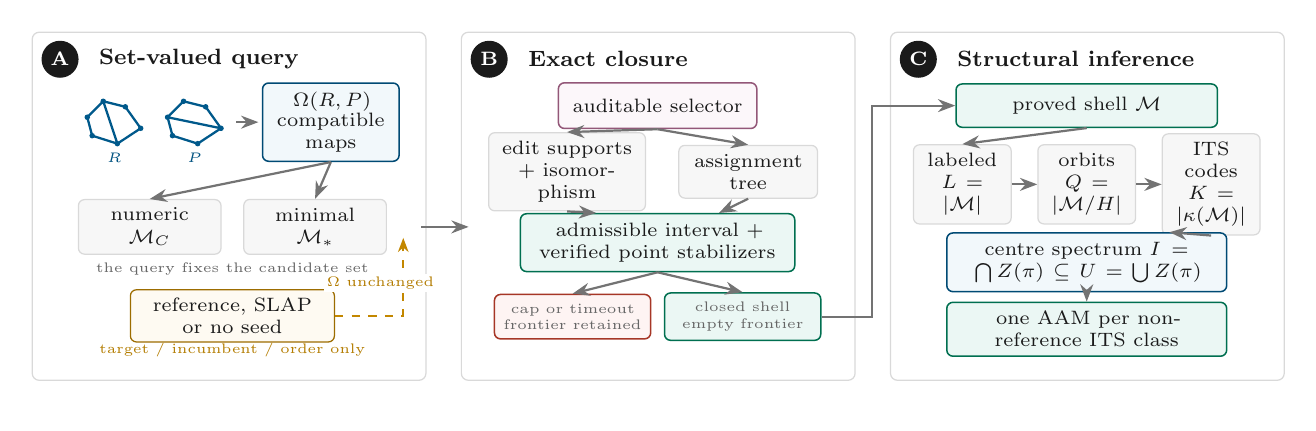
\begin{tikzpicture}[x=1cm,y=1cm]
  \path[use as bounding box] (0,-4.72) rectangle (16.0,0.05);

  \node[synpanel,minimum width=5.00cm,minimum height=4.42cm,
    anchor=north west] (panelA) at (0.05,0) {};
  \node[synpanel,minimum width=5.00cm,minimum height=4.42cm,
    anchor=north west] (panelB) at (5.50,0) {};
  \node[synpanel,minimum width=5.00cm,minimum height=4.42cm,
    anchor=north west] (panelC) at (10.95,0) {};
  \synpanelhead{0.24,-0.18}{A}{Set-valued query}
  \synpanelhead{5.69,-0.18}{B}{Exact closure}
  \synpanelhead{11.14,-0.18}{C}{Structural inference}

  % A. Endpoint data determine one immutable global assignment space.
  \begin{scope}[shift={(1.10,-1.15)},scale=.78]
    \draw[npgBlue!78!black,line width=.82pt]
      (-.44,.08)--(-.18,.34)--(.18,.25)--(.43,-.10)--(.05,-.35)
      --(-.36,-.22)--cycle (-.18,.34)--(.05,-.35);
    \foreach \p in {(-.44,.08),(-.18,.34),(.18,.25),(.43,-.10),
      (.05,-.35),(-.36,-.22)}
      \fill[npgBlue!78!black] \p circle (.045);
    \node[synsmall,text=npgBlue!72!black] at (0,-.58) {$R$};
  \end{scope}
  \begin{scope}[shift={(2.12,-1.15)},scale=.78]
    \draw[npgBlue!78!black,line width=.82pt]
      (-.44,.08)--(-.18,.34)--(.18,.25)--(.43,-.10)--(.05,-.35)
      --(-.36,-.22)--cycle (-.44,.08)--(.43,-.10);
    \foreach \p in {(-.44,.08),(-.18,.34),(.18,.25),(.43,-.10),
      (.05,-.35),(-.36,-.22)}
      \fill[npgBlue!78!black] \p circle (.045);
    \node[synsmall,text=npgBlue!72!black] at (0,-.58) {$P$};
  \end{scope}
  \draw[synflow] (2.65,-1.15)--(2.93,-1.15);
  \node[synquery,synlabel,text width=1.50cm,minimum height=.78cm]
    (omega) at (3.85,-1.15)
    {$\Omega(R,P)$\\[-1pt]\scriptsize compatible maps};

  \node[syncard,synlabel,text width=1.60cm,minimum height=.67cm]
    (numeric) at (1.55,-2.48) {numeric\\$\mathcal M_C$};
  \node[syncard,synlabel,text width=1.60cm,minimum height=.67cm]
    (minimum) at (3.65,-2.48) {minimal\\$\mathcal M_*$};
  \draw[synflow] (omega.south)--(numeric.north);
  \draw[synflow] (omega.south)--(minimum.north);
  \node[synsmall] at (2.60,-3.02)
    {the query fixes the candidate set};

  \node[syncard,synlabel,draw=npgOrange!68!black,fill=npgOrange!5,
    text width=2.38cm,minimum height=.55cm] (seed) at (2.60,-3.61)
    {reference, SLAP or no seed};
  \node[synsmall,text=npgOrange!78!black] at (2.60,-4.04)
    {target / incumbent / order only};

  % B. Both routes are exact; their selector changes work, not scope.
  \node[synmethod,synlabel,minimum width=2.52cm,minimum height=.58cm]
    (selector) at (8.00,-.94) {auditable selector};
  \node[syncard,synlabel,text width=1.78cm,minimum height=.67cm]
    (support) at (6.85,-1.78) {edit supports\\$+$ isomorphism};
  \node[syncard,synlabel,text width=1.55cm,minimum height=.67cm]
    (branch) at (9.15,-1.78) {assignment\\tree};
  \draw[synflow] (selector.south)--(support.north);
  \draw[synflow] (selector.south)--(branch.north);
  \node[synproof,synlabel,text width=3.25cm,minimum height=.64cm]
    (proof) at (8.00,-2.68)
    {admissible interval $+$\\verified point stabilizers};
  \node[synstop,synsmall,text width=1.75cm,minimum height=.52cm]
    (frontier) at (6.92,-3.62) {cap or timeout\\frontier retained};
  \node[synproof,synsmall,text width=1.75cm,minimum height=.52cm]
    (closed) at (9.08,-3.62) {closed shell\\empty frontier};
  \draw[synflow] (support.south)--([xshift=-.78cm]proof.north);
  \draw[synflow] (branch.south)--([xshift=.78cm]proof.north);
  \draw[synflow] (proof.south)--(frontier.north);
  \draw[synflow] (proof.south)--(closed.north);

  % C. Mapping, orbit and structural multiplicities remain distinct objects.
  \node[synproof,synlabel,minimum width=3.32cm,minimum height=.55cm]
    (shell) at (13.45,-.94) {proved shell $\mathcal M$};
  \node[syncard,synlabel,text width=1.03cm,minimum height=.77cm]
    (labeled) at (11.87,-1.94) {labeled\\$L=|\mathcal M|$};
  \node[syncard,synlabel,text width=1.03cm,minimum height=.77cm]
    (quotient) at (13.45,-1.94) {orbits\\$Q=|\mathcal M/H|$};
  \node[syncard,synlabel,text width=1.03cm,minimum height=.77cm]
    (classes) at (15.03,-1.94) {ITS codes\\$K=|\kappa(\mathcal M)|$};
  \draw[synflow] (shell.south)--(labeled.north);
  \draw[synflow] (labeled.east)--(quotient.west);
  \draw[synflow] (quotient.east)--(classes.west);
  \node[synquery,synlabel,text width=3.32cm,minimum height=.61cm]
    (centre) at (13.45,-2.93)
    {centre spectrum $I=\bigcap Z(\pi)\subseteq
      U=\bigcup Z(\pi)$};
  \draw[synflow] (classes.south)--([xshift=1.05cm]centre.north);
  \node[synproof,synlabel,text width=3.32cm,minimum height=.58cm]
    (alternatives) at (13.45,-3.78)
    {one AAM per non-reference ITS class};
  \draw[synflow] (centre.south)--(alternatives.north);

  % Solid arrows transmit scope/proof; the dashed seed arrow is advisory.
  \draw[synflow] (5.00,-2.48)--(5.60,-2.48);
  \draw[synhint] (seed.east)--(4.77,-3.61)--(4.77,-2.62);
  \node[synsmall,text=npgOrange!78!black,fill=white,inner sep=1pt]
    at (4.48,-3.19) {$\Omega$ unchanged};
  \draw[synflow] (closed.east)--(10.72,-3.62)--(10.72,-.94)--(shell.west);
\end{tikzpicture}
}
\caption{Formal inference contract of Synister.  \textbf{a}, Endpoint graphs
and atom compatibility define the global assignment space and the requested
numeric or minimal shell.  A supplied map can affect the target or traversal,
but the dashed advisory path cannot alter that space.  \textbf{b}, An
auditable selector chooses between two exact decompositions; bounds and
verified point stabilizers cover or reject the remaining assignment tree.
\textbf{c}, Only a closed shell supports exact labeled, symmetry-quotiented
and ITS-class multiplicities, invariant/possible centres and a
candidate-complete alternative-ITS panel.}
\label{fig:workflow}
\end{figure}

\section*{Results}

\subsection*{Atom mapping has a hard decision boundary and an exponential
output boundary}

Let $R$ and $P$ be balanced, undirected, atom-coloured endpoint graphs with
adjacency matrices $A$ and $B$, and let $\Omega(R,P)$ be their
colour-preserving bijections.  For every $\pi\in\Omega(R,P)$, Synister uses
\begin{equation}
 \CD(\pi)=\frac12\sum_{i,j}
  \left|A_{ij}-B_{\pi(i)\pi(j)}\right| .
 \label{eq:cd}
\end{equation}
The binary version is the edge symmetric difference; the weighted version
retains bond order.  A numeric shell is
$\mathcal M_C=\{\pi\in\Omega:\CD(\pi)=C\}$ and a minimal shell is
$\mathcal M_*=\mathcal M_{C^*}$ for
$C^*=\min_\pi\CD(\pi)$.

The decision problem ``is $\mathcal M_C$ non-empty?'' is NP-complete.  Thus
an algorithm that always closes arbitrary numeric shells efficiently would
solve an NP-complete problem.  The zero shell is the special coloured graph
isomorphism problem and is not known to be NP-complete.  Enumeration has a
separate, unavoidable output cost: even two empty $n$-vertex graphs have
$n!$ zero-distance labeled maps.  Synister consequently reports optimum proof,
enumeration completeness and output scope separately.  A timeout is not a
negative answer.

\subsection*{A hybrid exact algorithm exploits sparse chemical change}

For binary endpoints with $m_R$ and $m_P$ bonds, every map at distance $C$
breaks and forms exactly
\begin{equation}
 d_R=\frac{C+m_R-m_P}{2},\qquad
 d_P=\frac{C-m_R+m_P}{2}
 \label{eq:edit-budget}
\end{equation}
bonds.  Negative, non-integral or parity-inconsistent values certify an empty
shell immediately.  Otherwise Synister enumerates pairs of deleted edge
supports of these sizes and colour-preserving isomorphisms between the two
residual spanning graphs.  Each accepted map has one unique support pair, so
this is an exact decomposition rather than a candidate heuristic.  Its
selector estimate is
$\binom{m_R}{d_R}\binom{m_P}{d_P}$; the backend is used only below a declared
limit and only when labeled numeric-shell semantics are requested.

All other queries use assignment branch-and-bound.  The search maintains the
exact committed cost, incremental cross costs in $O(n^2)$ memory, element-wise
linear-assignment lower and upper bounds, and residual bond-mass bounds.  A
numeric branch is discarded when its attainable interval excludes the target.
Per-atom incident-bond profiles remove impossible assignments before search.
For a minimal shell, a first pass proves $C^*$ and a second pass streams only
maps at $C^*$, preventing provisional incumbents from reaching the output.
A Weisfeiler--Lehman-like sequential assignment mapper supplies a
reference-free feasible seed \citep{koda2025slapmapper}; the exact search
independently checks it and remains candidate-complete.

\begin{table}[t]
\centering
\caption{Mathematical scope of Synister outputs.  ``Complete'' always refers
to the stated row, never to an unstated larger space.}
\label{tab:scope}
\begin{tabular}{>{\raggedright\arraybackslash}p{0.25\linewidth}
                >{\raggedright\arraybackslash}p{0.31\linewidth}
                >{\raggedright\arraybackslash}p{0.34\linewidth}}
\toprule
Query & Candidate space & Completion claim \\
\midrule
Numeric global & all atom-compatible bijections at supplied $C$ & tolerance
shell $\mathcal M_{C,\varepsilon}$; equals $\mathcal M_C$ under the stated
lattice conditions \\
Minimal global & all atom-compatible bijections, then the minimum tolerance
shell & global minimum proved and $\mathcal M_{*,\varepsilon}$ exhausted;
equals $\mathcal M_*$ under the stated lattice conditions \\
Verified subgroup quotient & one stabilizer-chain representative per
$H\leq\Aut(P)$ orbit & exact only when the reported chain is complete \\
Reference-conditioned & declared fixed assignments plus free remainder &
exact within that conditioned subspace only \\
Interrupted & explored prefix tree and retained outputs & incomplete; never
promoted to a negative or complete result \\
\bottomrule
\end{tabular}
\end{table}

\subsection*{Verified symmetry separates multiplicity from structural
ambiguity}

Synister verifies every product-side permutation against the exact element
labels and objective matrix before using it.  Verified generators define a
subgroup $H\leq\Aut(P)$.  At depth $d$, candidates are partitioned by the
pointwise stabilizer of the previously chosen product images, and one candidate
per stabilizer orbit is visited.  If the bounded Schreier construction closes,
this yields one representative per $H$ orbit.  The action is free on complete
bijections, hence every orbit has size $|H|$ and the labeled count is the
representative count multiplied by $|H|$.  If construction does not close,
deeper symmetry pruning is disabled and quotient multiplicity is left unknown;
mapping completeness is never inferred from a partial chain.

Each retained map is also converted to a fully attributed ITS graph.  The
structural subgroup is required to preserve every unary property used by that
graph, in addition to atom colours and the product bond matrix.  Nodes
encode the element and before/after unary properties, while edges encode
before/after bond orders.  Exact coloured-graph canonicalization, rather than
a finite hash, defines structural identity.  A local template is induced by
changed atoms plus a stated union-graph radius; crossing bonds are retained as
boundary resource descriptors so context deletion cannot merge inequivalent
templates.  Synister reports labeled map multiplicity $L$, verified-subgroup
representative multiplicity $Q$, ITS richness $K$, verified-subgroup log
multiplicity $\log Q$, structural Hartley entropy $\log K$, and exact
bond/unary-atom change frequencies.  The first log quantity depends on the
reported subgroup unless the full automorphism group is proved.  The
intersection of changes is invariant across the shell in fixed reactant
coordinates; the union is the set of possible coordinate-level changes.

\subsection*{Pendant hydrogens can be eliminated exactly, but change the
global objective}

Assume that the two endpoints contain the same number of hydrogens, each a
degree-one leaf joined to one heavy atom by a unit bond.  For a fixed heavy map
$\pi$, let $r_i$ be the reactant hydrogen count at heavy atom $i$ and
$q_i=p_{\pi(i)}$ the product count transported by $\pi$.  Minimizing over all
explicit-hydrogen bijections $\sigma$ gives
\begin{equation}
 \min_\sigma \CD_{\mathrm{full}}(\pi,\sigma)
 =\CD_{\mathrm{heavy}}(\pi)+\sum_i|r_i-q_i|.
 \label{eq:hydrogen-factorization}
\end{equation}
Thus the explicit $H!$ hydrogen-permutation factor is unnecessary when only
the optimum score or its labeled multiplicity is required.  Synister computes
the minimum hydrogen contribution and its labeled multiplicity in closed form;
adding the heavy-atom CD gives the fixed-map full score.  Parent-indexed
transfer flows are enumerated only when individual plans are requested.

This is a conditional elimination, not permission to optimize heavy CD alone.
A three-atom path counterexample in the Supplementary Information has a
zero-heavy-CD map of full distance 6 but another heavy map of heavy CD 2 and
full distance 2.  Global additive full-atom optimization must therefore
minimize the combined right-hand side of
\cref{eq:hydrogen-factorization}, for example by adding the hydrogen term as a
unary assignment cost.  That combined branch-and-bound objective is not used
in the present release.  The FlowER pilot is explicitly a heavy-atom
bond-order-CD experiment; hydrogen-count changes are reported as unary centre
annotations rather than added to its score.

\subsection*{Independent exact controls recover the same mapping sets}

Correctness was tested as set equality, not only equality of optimum scores
(\cref{tab:validation}).  The support-first backend matched brute force for
every attainable shell of every pair of three-vertex simple graphs and for a
coloured five-vertex control.  Weighted four-vertex shells matched all 24
permutations with and without every enabled bound.  A relabelled five-cycle
regression is particularly diagnostic: global orbit sorting, an unsafe rule
in earlier solvers, loses the true optimum.  Stabilizer branching returns one
representative, its verified group order is ten, and expansion equals the ten
labeled isomorphisms exactly.  Directed-matrix and stale-symmetry regressions
verify that a visually plausible undirected automorphism cannot alter the
objective.

\begin{table}[t]
\centering
\caption{Exact validation performed under a hard 6 GiB address-space cap and
one numerical thread.  The count includes the available PuLP/CBC integration
control.}
\label{tab:validation}
\begin{tabular}{>{\raggedright\arraybackslash}p{0.36\linewidth}
                >{\raggedright\arraybackslash}p{0.48\linewidth}}
\toprule
Control & Result \\
\midrule
All pairs of simple graphs on three vertices & edit-support mappings equal
brute-force mappings for every non-empty shell \\
Weighted four-vertex pair & minimum and every numeric shell equal all 24
brute-force permutations \\
Relabelled $C_5$ & CD minimum 0; 10 labeled maps; 1 representative under a
verified order-10 subgroup \\
Streaming, caps and zero-time interruption & counts/digests agree; incomplete
status never becomes a proof \\
Mapper and validator suite & 102 passed, including the MILP control; maximum
resident set 205,508 KiB; zero swap \\
\bottomrule
\end{tabular}
\end{table}

\subsection*{Blinded FlowER reactions reveal structural degeneracy}

We froze a resource-censored pilot comprising the first 100 rows processed in
file order from a result-independent 10,000-row FlowER test cohort
\citep{joung2025flower,flowerdata}.  Reactant and product atom
orders were independently permuted using different deterministic salts.  The
held-out map was not passed to either exact search.  Reference-CD mode used
only its scalar distance; minimal mode hid both map and distance.  Each shell
shell call had a one-second cooperative budget; streamed minimal queries
used separate optimization and enumeration passes within that outer budget.
The process used one
worker and one numerical thread, and its address space was capped at 6 GiB.
The 100 case identities, case records, manifest and digests are frozen with
the manuscript.  All conditional fractions below use closed shells only and
are not estimates for the 10,000-row cohort or the full FlowER population.

\begin{figure}[H]
\centering
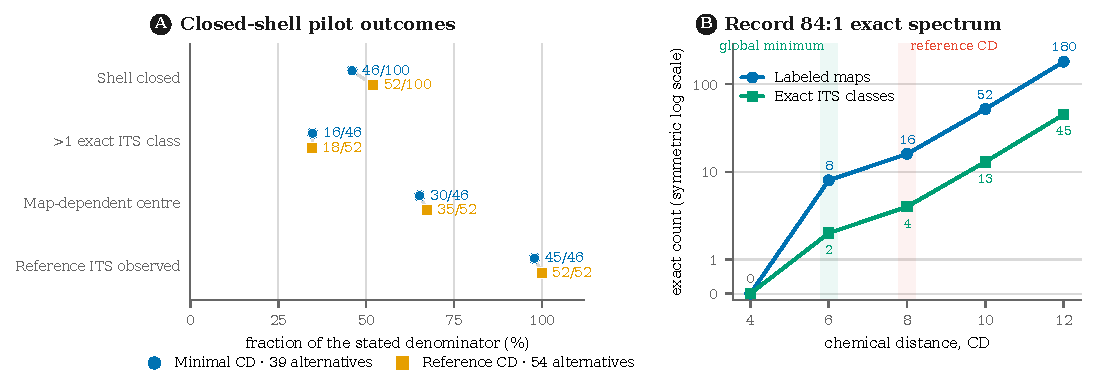
\includegraphics[width=\linewidth]{figures/pilot_spectrum.pdf}
\caption{Exact-shell evidence. \textbf{a}, Reference-blinded FlowER pilot.
Closure uses all 100 attempted reactions; other fractions use only closed
shells.  Timeouts are censored, not scored as negatives.  Legend totals count
exact ITS classes different from the held-out reference. \textbf{b}, Complete
numeric shells for record 84:1.  Point labels are exact counts; the
symmetric-log axis includes the certified empty CD-4 shell.  All three seed
modes produced the same class sets.}
\label{fig:pilot}
\end{figure}

Forty-six minimal shells and 52 reference-CD shells closed
(\cref{fig:pilot}).  All 46 closed minimal shells contained more than one
labeled map, with a median of 16 and a maximum of 192.  Symmetry did not explain
all ambiguity: 16 of the 46 contained multiple exact ITS classes (up to 16),
and the same 16 contained multiple boundary-aware template classes.  In fixed
reactant coordinates, 30 had a reaction-centre union larger than its
intersection.  Thus arbitrary single-map selection would alter at least one
coordinate-level atom or bond label in 30 closed cases, even though every
selected map had globally minimal heavy-atom CD.  The 16 non-isomorphic ITS
sets, rather than the coordinate count alone, establish structural ambiguity.
Relative to the held-out ITS, those 16 cases yielded 39 exact alternative ITS
classes.  The 18 ambiguous reference-CD cases yielded 54.  Selecting one
representative AAM from each class under a fixed recorded traversal therefore
gives a candidate-complete contrastive panel for every closed shell, rather
than unverified random atom permutations.  Class identifiers and class sets
are seed-invariant; the labeled representative need not be.

The held-out reference ITS class appeared in 45 of 46 closed minimal shells.
In FlowER record 84:1 (source line 109; 13 heavy atoms), its heavy-atom CD was
8, whereas Synister proved a global minimum of 6 with eight labeled maps, two
verified-subgroup representatives and two non-isomorphic ITS classes.  This
is not an annotation-error claim: it is direct evidence that endpoint CD and
the dataset reference correspondence need not define the same preference.
Reference-CD mode closed the supplied shell for 52 cases and recovered the
reference class in all 52, as required of a successful completeness control.
For record 84:1, additional numeric shells at CD 4, 6, 10 and 12 also closed:
they contained respectively 0, 8, 52 and 180 labeled maps and 0, 2, 13 and 45
exact ITS classes.  Reference, reference-free SLAP and no-seed runs agreed on
every class set, although the labeled representative selected within a class
could differ.  Their node counts differed non-monotonically, so a dataset reference
can supply a target or incumbent but is not a guaranteed acceleration.

\section*{Discussion}

Atom mapping is both computationally hard and scientifically set-valued.
These are not excuses for opacity.  They determine what a defensible mapper
must report: the precise candidate space, whether the optimum is proved,
whether its shell is exhausted, which symmetry group was verified, how many
labeled and structural alternatives remain, and why a computation stopped.
Synister provides these quantities in one exact interface.

The closed pilot shells establish a consequence relevant beyond mapping
algorithms.  All 46 closed minimum shells contained multiple labeled maps, but
only 16 contained multiple ITS classes; raw mapping counts can therefore
overstate structural uncertainty.  Conversely, those 16 contained genuinely
non-isomorphic endpoint transformations, and 30 had coordinate-level centre
instability, so one arbitrary map can still alter a downstream label.
Template databases and mapping-dependent learning systems can inherit that
choice from preprocessing.  Synister exports one AAM per exact non-reference
ITS class, providing candidate-complete contrastive panels for future
invariant-label training or ambiguity-aware evaluation.  Here ``alternative''
means different from the reference ITS under the declared endpoint score; it
does not assert mechanistic impossibility or annotation error.

The present evidence has deliberate limits.  Closure under the cooperative
per-shell-call budget is selected by computational difficulty, so the conditional
pilot fractions cannot be generalized to 10,000 reactions.  The centre unions
are defined in fixed reactant coordinates and are not a reactant-symmetry
quotient.  Heavy-atom CD is a structural objective, not a complete mechanism
or energetic model, and the implemented post hoc hydrogen lift is not a global
full-CD optimizer.  No universal runtime gain follows from eliminating $H!$:
the remaining heavy-map problem is NP-hard and explicit output can still be
factorial.  Larger preregistered resource strata, matched-objective performance
and ablation benchmarks, expert mechanistic comparisons and downstream model
tests are needed before population, speed or predictive-benefit claims.

\section*{Methods}

\subsection*{Graph representation and query policy}

Write the endpoints as $R=(V_R,A,\chi_R,u_R)$ and
$P=(V_P,B,\chi_P,u_P)$, where $A,B\in\mathbb R_{\geq0}^{n\times n}$ are bond
matrices, $\chi$ is the immutable assignment colour and $u$ contains declared
unary attributes used for symmetry or structural identity.  Molecular inputs
have symmetric matrices with zero diagonal; self-loops are excluded.  Weighted
mode retains bond order and binary mode replaces every non-zero bond by one.
The global assignment space is
\begin{equation}
 \Omega(R,P)=\{\pi:V_R\overset{\sim}{\longrightarrow}V_P:
 \chi_R(i)=\chi_P(\pi(i))\ \text{for all }i\}.
 \label{eq:assignment-space}
\end{equation}
The endpoints are balanced when every colour has equal multiplicity $n_e$ on
both sides, in which case $|\Omega|=\prod_e n_e!$; otherwise $\Omega$ is empty.
The present molecular adapter uses atomic number for $\chi$.

The mathematical shells use exact rational weights.  For arbitrary
floating-point inputs the implementation instead closes the declared
tolerance shell
$\mathcal M_{C,\varepsilon}=\{\pi:|\CD(\pi)-C|\leq\varepsilon\}$, and minimal
mode retains every map within $\varepsilon$ of the computed optimum.  Binary
weights and the pilot's verified $\{1,1.5,2,3\}$ bond orders lie on an exactly
representable half-integer cost lattice.  The pilot's numeric targets also lie
on that lattice, and with $\varepsilon=10^{-9}<0.25$ its tolerance shells equal
the algebraic shells.  No such equality is claimed for an off-lattice target
or unrestricted user-supplied real weights.

A numeric global query returns $\mathcal M_{C,\varepsilon}\subseteq\Omega$ and
a minimal global query first proves $C^*$ and then returns
$\mathcal M_{*,\varepsilon}$.  Under the lattice conditions above these are
$\mathcal M_C$ and $\mathcal M_*$, respectively.  For a declared compatible
partial map $F$, a conditioned query instead searches
$\Omega_F=\{\pi\in\Omega:\pi(i)=F(i)\text{ for }i\in\operatorname{supp}F\}$.
Completeness in $\Omega_F$ is not global completeness unless
$\mathcal M_C\subseteq\Omega_F$ is independently proved.  A
reference-assisted global query may use a map to define $C$, seed an incumbent
or order traversal, but it never constructs $F$.  In the blinded pipeline,
mapped SMILES are parsed only to recover a held-out correspondence; endpoint
orders are independently permuted, the correspondence remains outside the
search call and the SLAP seed is computed from blinded endpoints alone.

Every result separates mathematical scope from termination state.
\texttt{complete} closes a non-empty declared mapping shell,
\texttt{no\_solutions} closes an empty one, and \texttt{timeout} retains an
unresolved mapping frontier after a search or output cap.  Quotient-chain and
ITS/template classification completeness are separate fields: a subordinate
cap can leave the mapping shell closed while the downstream classification is
incomplete.  Only the corresponding completed field supports its exhaustion
claim.

\subsection*{Complexity of exact-shell mapping}

\begin{theorem}[Exact-shell complexity]
Given two simple vertex-coloured graphs with equal colour multiplicities and a
non-negative integer $C$, deciding whether $\mathcal M_C$ is non-empty is
NP-complete.  Deciding whether some map has CD at most $K$ is NP-complete, and
minimum-CD optimization is NP-hard.  The restriction $C=0$ is coloured graph
isomorphism.
\end{theorem}

\begin{proof}
Membership in NP follows because a proposed colour-preserving bijection and
its value under \cref{eq:cd} are checked in polynomial time.  For hardness,
reduce from \textsc{Clique}
\citep{karp1972reducibility}.  Given a graph $G$ on $n$ vertices and an integer
$k$, let $R=G$ and let $P$ be the disjoint union of $K_k$ and $n-k$ isolated
vertices; give every vertex the same colour.  Write $m=|E(G)|$ and
$c=\binom{k}{2}$.  Every bijection selects the $k$-vertex preimage $S$ of the
product clique and has
\[
 \CD(\pi)=m+c-2|E(G[S])|.
\]
If $m\geq c$, then $|E(G[S])|\leq c$ and equality
$\CD(\pi)=m-c$ holds precisely when $S$ is a $k$-clique; the same value is the
smallest possible threshold.  If $m<c$, the Clique instance is necessarily
negative and is mapped to a fixed negative instance.  This proves exact-shell
and threshold hardness, and the optimization claim follows.  At $C=0$, the
question is exactly coloured graph isomorphism, whose NP-completeness is not
known.
\end{proof}

The same construction shows why counting is harder than finding one map.  For
each $k$-clique, exactly $k!(n-k)!$ bijections attain $m-c$.  Thus exact-shell
counting recovers the number of $k$-cliques after division by a known factor;
it is \#P-hard and lies in \#P.  Explicit enumeration has lower bound
$\Omega(Ln)$ for $L$ length-$n$ labeled outputs.  A polynomial-delay enumerator
that also certified every empty numeric shell in polynomial time would imply
$\mathrm P=\mathrm{NP}$.

\subsection*{Binary edit-support decomposition}

For a map $\pi$, let $D_R(\pi)$ be reactant edges absent after transport from
the product, and let $D_P(\pi)$ be transported product edges absent from the
reactant.  Binary CD is $|D_R|+|D_P|$, while edge-count balance gives
$m_R-|D_R|=m_P-|D_P|$.  Solving these equations yields
\cref{eq:edit-budget}.

\begin{proposition}
For feasible $d_R,d_P$, mappings in $\mathcal M_C$ are in bijection with
triples $(D_R,D_P,\phi)$ where $|D_R|=d_R$, $|D_P|=d_P$, and $\phi$ is a
colour-preserving isomorphism $R-D_R\cong P-D_P$ whose mismatch sets in the
original endpoints are exactly $D_R,D_P$.
\end{proposition}

\begin{proof}
Deleting the two mismatch sets from a shell mapping leaves precisely the
conserved edges, so the mapping restricts to the required spanning-graph
isomorphism.  Conversely, rescoring an accepted isomorphism against the
original endpoints gives $d_R+d_P=C$.  The mismatch sets are functions of the
mapping, establishing uniqueness and preventing duplicates across support
pairs.
\end{proof}

Residual graphs are bucketed by collision-tolerant invariants before exact
NetworkX isomorphism.  Every isomorphism is independently rescored.  Support,
mapping and time caps return incomplete results.  The automatic selector uses
this route only for binary numeric labeled shells, without certificates, fixed
assignments or symmetry quotienting, and only when the support estimate is at
most the configured threshold.  The recorded decision includes the estimate,
limit, selected backend and reason.

\subsection*{Assignment branch-and-bound}

Fix a deterministic reactant order.  At a search prefix, let $S,T$ be the
assigned reactant and product vertices, let $U,V$ be the remaining vertices
and let $c(S,T)$ contain the exact assigned--assigned cost.  For a compatible
remaining pair $(i,p)$, the exact interaction with the prefix is
\begin{equation}
 X_{ip}=\frac12\sum_{j\in S}
 \left(|A_{ij}-B_{p,\pi(j)}|+|A_{ji}-B_{\pi(j),p}|\right).
 \label{eq:cross-cost}
\end{equation}
The full $n\times n$ array $X$ is updated and undone incrementally, requiring
$O(n^2)$ working memory rather than an $O(n^4)$ pair tensor.  Let $L_X$ and
$U_X$ be the sums, over colour blocks, of the minimum and maximum compatible
linear assignments in $X$.  For residual matrix sums
$a_U=\sum_{i,j\in U}A_{ij}$ and $b_V=\sum_{p,q\in V}B_{pq}$, and absolute sums
$\alpha_U,\beta_V$, every completion of the prefix satisfies
\begin{equation}
 c(S,T)+L_X+\frac12|a_U-b_V|
 \;\leq\;\CD(\pi)\;\leq\;
 c(S,T)+U_X+\frac12(\alpha_U+\beta_V).
 \label{eq:subtree-interval}
\end{equation}
The assignment extrema bound every feasible residual bijection, and the
internal terms follow from the reverse and ordinary triangle inequalities.
A numeric branch is rejected exactly when its target lies outside this
interval; minimization compares the lower endpoint with a verified incumbent.
Sorted incident-bond profiles within neighbour-colour blocks provide a
second admissible pairwise lower bound and remove only assignments already
incapable of reaching the numeric target.

Candidate images are tried according to incremental cost and then the declared
seed.  Reactant atoms are ordered from the seed's changed centre outward, with
rare elements and higher degree breaking ties.  These choices affect traversal
only.  Minimal streaming uses two logically separate passes: the first proves
the global incumbent, and the second fixes that value and invokes callbacks
only for $\mathcal M_*$.  Numeric-shell users may omit optimization when they
request only $\mathcal M_C$.

\subsection*{Exact symmetry compression}

Canonical graph search returns concrete product automorphisms under explicit
time and node limits \citep{mckay2014nauty}.  Every candidate permutation is
then checked by exact equality of atom colours and all objective-matrix
entries.  For structure-spectrum analyses, the checked colour also contains
every product unary property used by reaction-centre or ITS identity.  Thus
the structural subgroup lies in $\Aut(P;B,\chi,u)$, not merely the un-attributed
bond-graph automorphism group.  Cache keys include a digest of the checked
graph data.  Failure or bounded termination yields the identity subgroup,
which can reduce speed but cannot remove a mapping.

Let verified generators define $H\leq\Aut(P)$ acting by
$(h\cdot\pi)(i)=h(\pi(i))$.  The action preserves CD.  At a prefix with images
$y_1,\ldots,y_{d-1}$, Synister computes generators for
$\Stab_H(y_1,\ldots,y_{d-1})$, partitions the next candidate domain into its
orbits and visits the least member of each orbit.

\begin{proposition}
If every stabilizer construction is complete, orbital branching visits exactly
one leaf per $H$ orbit.  The action of $H$ on complete bijections is free.
\end{proposition}

\begin{proof}
Canonical augmentation gives existence by repeatedly transporting the first
non-canonical choice with a stabilizer element that fixes the earlier prefix.
For uniqueness, two retained equivalent leaves have a first differing
position; their common earlier prefix forces the relating element into that
prefix stabilizer, contradicting retention of two candidates from one orbit.
If $h\circ\pi=\pi$, surjectivity of $\pi$ implies $h$ fixes every product
vertex, hence $h$ is the identity.
\end{proof}

The subgroup order is computed through bounded Schreier stabilizers without
materializing all group elements.  A work-budget exit disables deeper pruning
and sets quotient completeness false.  Full labeled output is available by
running without quotienting; a fully enumerated verified cyclic subgroup may
also be expanded exactly once per representative.

\subsection*{Reaction-centre and structure spectra}

For mapping $\pi$, define
$\Delta^\pi_{ij}=B_{\pi(i),\pi(j)}-A_{ij}$.  At declared absolute tolerance
$\varepsilon$, let $Z_\varepsilon(\pi)$ be the disjoint, type-tagged union of
bonds with $|\Delta^\pi_{ij}|>\varepsilon$ and atoms whose declared transported
unary properties change.  For a closed reported shell $\mathcal M$, the
invariant and possible reaction centres are
\begin{equation}
 I_\varepsilon(\mathcal M)=\bigcap_{\pi\in\mathcal M}Z_\varepsilon(\pi),\qquad
 U_\varepsilon(\mathcal M)=\bigcup_{\pi\in\mathcal M}Z_\varepsilon(\pi).
 \label{eq:centre-spectrum}
\end{equation}
Thus $U_\varepsilon\setminus I_\varepsilon$ is precisely the
mapping-dependent region in the fixed reactant indexing; exact counters
separately give each bond and unary-atom change frequency.  On a lattice whose
smallest non-zero bond change exceeds $\varepsilon$, this is the algebraic
non-zero support.  This coordinate statistic is not a quotient by reactant
automorphisms.  A deterministic digest commits to the representative stream.

Full ITS and radius-$r$ template graphs are canonicalized with SynKit's exact
coloured-graph canonicalizer.  Template node colours include a sorted
description of bonds crossing the retained boundary: outside element, before
order and after order.  Canonical codes are injective serializations of the
exact certificate; SHA-256 values are identifiers only and are never used to
assert identity.  A canonicalization timeout marks structure analysis
incomplete without changing the independently established mapping-shell
status.

Let $\kappa(\pi)$ be the exact canonical ITS code and
$\mathcal K(\mathcal M)=\{\kappa(\pi):\pi\in\mathcal M\}$.  Maps in one
product-side $H$ orbit induce isomorphic ITS graphs, so complete quotienting
preserves $\mathcal K$; freeness and the common orbit size $|H|$ also preserve
normalized class frequencies.  A shell has one structural class exactly when
$|\mathcal K|=1$, whereas its fixed-coordinate centre is map-invariant exactly
when $I_\varepsilon=U_\varepsilon$; neither condition follows from the other by
definition.

For reference map $\pi_0$, the alternative panel at target $C$ contains one
reproducibly selected AAM per code, for a fixed seed and configuration, in
$\mathcal K(\mathcal M_C)\setminus\{\kappa(\pi_0)\}$.  Product-orbit pruning
preserves this set by the invariance above.  The application reports
completeness only when both the global mapping shell and every requested
canonicalization close; otherwise observed representatives remain explicitly
incomplete.

\subsection*{Hydrogen-flow lifting}

The factorization assumes balanced hydrogen inventories; degree-one,
unit-bonded hydrogen leaves; hydrogen-to-hydrogen compatibility; and no
H--H, bridging, multicentre or isotope-specific terms.  An inventory imbalance
is rejected rather than silently padded.  For fixed $\pi$, a hydrogen flow
$X=(x_{ij})$ has row sums $r_i$ and column sums $q_j=p_{\pi(j)}$.  Its exact
decomposition is
\[
 \CD_{\mathrm{full}}(\pi,X)=\CD_{\mathrm{heavy}}(\pi)
   +2\bigl(H-\operatorname{tr}X\bigr).
\]
Every minimum flow has $x_{ii}=\min(r_i,q_i)$, so
$T=\tfrac12\sum_i|r_i-q_i|$ hydrogens change parent.  A particular flow has
labeled multiplicity
$N(X)=\prod_i r_i!\prod_jq_j!/\prod_{i,j}x_{ij}!$.  Summing over all minimum
flows gives the closed form
\begin{equation}
 L_H(\pi)=T!\prod_i
 \frac{\max(r_i,q_i)!}{|r_i-q_i|!}.
 \label{eq:hydrogen-multiplicity}
\end{equation}
The implementation evaluates the minimum hydrogen contribution and $L_H$ in
linear time in the number of heavy parents, apart from big-integer arithmetic.
It enumerates
parent-indexed flow matrices only on request; a plan cap makes that enumeration
incomplete.  Global full-CD minimization would additionally require minimizing
\cref{eq:hydrogen-factorization} over all heavy maps.  Arbitrary nonminimum
numeric full-CD shells also require nonminimum hydrogen lifts and are outside
this conditional routine.

\subsection*{Validation and FlowER pilot}

Brute-force tests enumerate atom-compatible permutations directly.  Backend
acceptance requires equality of complete mapping sets for every shell, equality
of minimum values and optimizer sets, exact expansion of symmetry quotients,
and fail-closed behavior under caps, timeouts and tampered certificates.  The
exact acceptance command, dependency environment and resource record are given
in the Supplementary Information; no frozen pilot case is represented as an
independently replayed prefix certificate.

The FlowER pilot used the frozen file digest in
\path{paper/synister/evidence/pilot100_v4/manifest.json}.  One hundred case
records were processed sequentially in file order.  Each shell call had a
one-second cooperative budget.  Streamed minimal mode used a prerequisite
optimization pass followed by an enumeration pass with only the time remaining
in that same outer budget.  The 10,000-output cap,
0.25-second symmetry-discovery bound and 0.1-second per-representative structure
bound were separate.  The whole process used 188.68 seconds wall time and
peaked at 293,772 KiB resident memory.  The standalone manuscript summarizer
recomputed the manifest, payload and case-to-manifest digests before deriving
statistics.  A case contributes to a denominator only if both mapping
enumeration and the statistic being reported are complete.

The alternative-ITS application reprocessed record 84:1 at the global minimum,
the reference CD and four numeric CDs, each with reference, SLAP and no seed.
All 18 queries closed under a 6 GiB cap and one thread, peaked at 217,404 KiB,
and agreed across seed modes on status, labeled count and exact class set.  Its
record binds the dataset, reaction and historical selected-file digest and
exports AAM correspondences without redistributing the reaction.

\subsection*{Statistics and reproducibility}

The unit of analysis was one reaction row.  The pilot size of 100 was a
resource-bounded development choice, not a power calculation; rows were the
first 100 processed from the frozen cohort in file order, with no random
sampling or post-outcome replacement.  Endpoint atom orders were blinded by a
deterministic salt before search.  No hypothesis tests, confidence intervals,
randomization or imputation were used.  Closure rates use all 100 attempts;
other denominators require a closed mapping shell and complete requested
structure analysis.  Timeouts and caps are right-censored incomplete outcomes,
not negatives.  All reported counts are exact descriptive counts of these
frozen records, not population estimates.

OpenAI Codex was used for code review, test development, mathematical and
language editing during manuscript revision.  The author reviewed the changes,
reran the reported validation and retains responsibility for the manuscript
and software.

\section*{Data availability}

The original FlowER dataset is available from Figshare under its original
terms \citep{flowerdata}.  The analyzed result-independent 10,000-row cohort is
tracked in the companion Synister repository at commit \texttt{900d40e}; its
SHA-256 digest is:
\begin{center}\small
\texttt{e40647847169a7fc98af1aab44fa81c7a64deb70b77085ae3deb3925e39642b0}
\end{center}
The manuscript evidence directory contains the 100 frozen row identities,
campaign manifest, reference-blinded case records, resource record, derived
censored summary and alternative-ITS case study.  The case records themselves
contain neither reaction SMILES nor raw reference mappings.  An archival DOI
for generated evidence remains to be supplied before publication.

\section*{Code availability}

All active implementation, tests and campaign scripts are in the MIT-licensed
SynKit repository \citep{synkit}; the method retains the name Synister.  The
repository includes an installation specification, tests, bounded examples
and machine-readable backend decisions.  Frozen campaign records carry the
historical digest of a selected campaign-critical file set; that digest is not
a whole-repository hash and does not match the evolving current source.  A
tagged archival release and DOI, together with the final Git commit and replay
environment, remain to be supplied before publication.

\section*{Acknowledgements}

The author thanks the developers of the open-source software used in this
work.

\section*{Funding}

Funding information must be supplied by the author before submission.

\section*{Author contributions}

T.-L.P. conceived the study, developed the method, performed the analysis and
wrote the manuscript.

\section*{Competing interests}

The author declares no competing interests.

{\small
\bibliographystyle{unsrtnat}
\bibliography{ref}
}

\end{document}
